% questions.tex —— 2021 年·全国甲卷·理科 · 题目内容片段（无答案）
% 由 tools/generate_projects.py 依来源总账自 2021/2021_数学真题_全国甲理_试题.md 生成，勿手改（改源 MD 后重跑）


\gkpart{数学}

\begin{gktip}
\textbf{结构提示}：本卷共 23 题。第 1～12 题为选择题，第 13～16 题为填空题；第 17～21 题为必考解答题，第 22、23 题为选考题（二选一）。
\end{gktip}

\par\medskip

\gkpart{一、选择题}

\begin{gktip}
本题共 12 小题，每小题 5 分，共 60 分。在每小题给出的四个选项中，只有一项是符合题目要求的。
\end{gktip}

\begin{question}
\gkti{1}设集合 $M=\{x\mid 0<x<4\}$，$N=\left\{x\mid \dfrac13\leqslant x\leqslant5\right\}$，则 $M\cap N=$\mbox{（　　）}

\begin{gkopts}(2)
\task A．$\left\{x\mid 0<x\leqslant\dfrac13\right\}$
\task B．$\left\{x\mid\dfrac13\leqslant x<4\right\}$
\task C．$\{x\mid4\leqslant x<5\}$
\task D．$\{x\mid0<x\leqslant5\}$
\end{gkopts}

\Needspace{0.4\textheight}
\end{question}
\begin{question}
\gkti{2}为了解某地农村经济情况，对该地农户家庭年收入进行抽样调查，将农户家庭年收入的调查数据整理得到如下频率分布直方图：
\nopagebreak[4]
\begin{center}% 2021 全国甲卷理科 2：农村家庭年收入频率分布直方图
% 根据固定上游 PDF 第 1 页：组距均为 1，组界 2.5 至 14.5。
% 各柱高依次为 0.02, 0.04, 0.10, 0.14, 0.20, 0.20, 0.10, 0.10, 0.04, 0.02, 0.02, 0.02。
\begin{tikzpicture}[font=\small]
  \def\xs{0.48}\def\ys{15.0}\def\xz{0.52}
  % 横轴断轴与纵轴
  \draw (0,0) -- (0.10,0);
  \draw (0.10,0) -- (0.16,0.09) -- (0.25,-0.09) -- (0.31,0);
  \draw[->] (0.31,0) -- ({\xz+12*\xs+0.55},0);
  \draw[->] (0,0) -- (0,{0.20*\ys+0.45});
  \node[anchor=north] at (0,-0.04) {$0$};
  \node[anchor=south east,align=center] at (-0.04,{0.20*\ys+0.1}) {频率/组距};
  \node[anchor=west] at ({\xz+12*\xs+0.2},0.15) {收入/万元};
  % 刻度参考线及标注
  \foreach \v in {0.02,0.04,0.10,0.14,0.20} {
    \draw[densely dotted,gray!70] (0,{\v*\ys}) -- ({\xz+12*\xs},{\v*\ys});
    \node[anchor=east,inner sep=2pt,font=\scriptsize] at (-0.04,{\v*\ys}) {$\v$};
  }
  % 十二组柱形
  \foreach \i/\h in {0/0.02,1/0.04,2/0.10,3/0.14,4/0.20,5/0.20,
                       6/0.10,7/0.10,8/0.04,9/0.02,10/0.02,11/0.02} {
    \draw ({\xz+\i*\xs},0) rectangle ({\xz+(\i+1)*\xs},{\h*\ys});
  }
  \foreach \i/\xlab in {0/2.5,1/3.5,2/4.5,3/5.5,4/6.5,5/7.5,6/8.5,
                         7/9.5,8/10.5,9/11.5,10/12.5,11/13.5,12/14.5} {
    \node[anchor=north,inner sep=1pt,font=\tiny] at ({\xz+\i*\xs},-0.04) {$\xlab$};
  }
\end{tikzpicture}
\end{center}
\nopagebreak[4]
根据此频率分布直方图，下面结论中不正确的是\mbox{（　　）}

\begin{gkopts}(1)
\task A．该地农户家庭年收入低于 $4.5$ 万元的农户比率估计为 $6\%$
\task B．该地农户家庭年收入不低于 $10.5$ 万元的农户比率估计为 $10\%$
\task C．估计该地农户家庭年收入的平均值不超过 $6.5$ 万元
\task D．估计该地有一半以上的农户，其家庭年收入介于 $4.5$ 万元至 $8.5$ 万元之间
\end{gkopts}

\end{question}
\begin{question}
\gkti{3}已知 $(1-\mathrm i)^2z=3+2\mathrm i$，则 $z=$\mbox{（　　）}

\begin{gkopts}(2)
\task A．$-1-\dfrac32\mathrm i$
\task B．$-1+\dfrac32\mathrm i$
\task C．$-\dfrac32+\mathrm i$
\task D．$-\dfrac32-\mathrm i$
\end{gkopts}

\end{question}
\begin{question}
\gkti{4}青少年视力是社会普遍关注的问题，视力情况可借助视力表测量。通常用五分记录法和小数记录法记录视力数据，五分记录法的数据 $L$ 和小数记录法的数据 $V$ 满足 $L=5+\lg V$。已知某同学视力的五分记录分的数据为 $4.9$，则其视力的小数记录法的数据约为（$\sqrt[10]{10}\approx1.259$）\mbox{（　　）}

\begin{gkopts}(4)
\task A．$1.5$
\task B．$1.2$
\task C．$0.8$
\task D．$0.6$
\end{gkopts}

\end{question}
\begin{question}
\gkti{5}已知 $F_1$，$F_2$ 是双曲线 $C$ 的两个焦点，$P$ 为 $C$ 上一点，且 $\angle F_1PF_2=60^\circ$，$|PF_1|=3|PF_2|$，则 $C$ 的离心率为\mbox{（　　）}

\begin{gkopts}(2)
\task A．$\dfrac{\sqrt7}{2}$
\task B．$\dfrac{\sqrt{13}}2$
\task C．$\sqrt7$
\task D．$\sqrt{13}$
\end{gkopts}

\Needspace{0.4\textheight}
\end{question}
\begin{question}
\gkti{6}在一个正方体中，过顶点 $A$ 的三条棱的中点分别为 $E$，$F$，$G$。该正方体截去三棱锥 $A\text{-}EFG$ 后，所得多面体的三视图中，正视图如图所示，则相应的侧视图是\mbox{（　　）}
\nopagebreak[4]
\begin{center}% 2021 全国甲卷理科 6：正视图与四个备选侧视图
% 依据固定上游 PDF 第 1 页。切口投影均落在方形边的中点；虚线/实线按遮挡关系区分。
\begin{tikzpicture}[font=\small,line width=0.4pt]
  \def\s{1.38}
  \newcommand{\cutleft}[1][]{\draw[#1] (0,{0.5*\s}) -- ({0.5*\s},0);}
  \newcommand{\cutright}[1][]{\draw[#1] ({0.5*\s},0) -- (\s,{0.5*\s});}
  % 正视图
  \begin{scope}[shift={({2.15*\s},{1.18*\s})}]
    \draw (0,0) rectangle (\s,\s);
    \cutleft[dashed]
    \node[anchor=south] at ({0.5*\s},\s+0.04) {正视图};
  \end{scope}
  % A：右下角、实线
  \begin{scope}[shift={(0,0)}]
    \draw (0,0) rectangle (\s,\s); \cutright
    \node[anchor=east] at (-0.05,{0.06*\s}) {A};
  \end{scope}
  % B：左下角、虚线
  \begin{scope}[shift={({1.55*\s},0)}]
    \draw (0,0) rectangle (\s,\s); \cutleft[dashed]
    \node[anchor=east] at (-0.05,{0.06*\s}) {B};
  \end{scope}
  % C：右下角、虚线
  \begin{scope}[shift={({3.10*\s},0)}]
    \draw (0,0) rectangle (\s,\s); \cutright[dashed]
    \node[anchor=east] at (-0.05,{0.06*\s}) {C};
  \end{scope}
  % D：左下角、实线
  \begin{scope}[shift={({4.65*\s},0)}]
    \draw (0,0) rectangle (\s,\s); \cutleft
    \node[anchor=east] at (-0.05,{0.06*\s}) {D};
  \end{scope}
\end{tikzpicture}
\end{center}
\nopagebreak[4]
\end{question}
\begin{question}
\gkti{7}等比数列 $\{a_n\}$ 的公比为 $q$，前 $n$ 项和为 $S_n$。设甲：$q>0$，乙：$\{S_n\}$ 是递增数列，则\mbox{（　　）}

\begin{gkopts}(2)
\task A．甲是乙的充分条件但不是必要条件
\task B．甲是乙的必要条件但不是充分条件
\task C．甲是乙的充要条件
\task D．甲既不是乙的充分条件也不是乙的必要条件
\end{gkopts}

\Needspace{0.4\textheight}
\end{question}
\begin{question}
\gkti{8}2020 年 12 月 8 日，中国和尼泊尔联合公布珠穆朗玛峰最新高程为 $8848.86$（单位：m）。三角高程测量法是珠峰高程测量方法之一。如图是三角高程测量法的一个示意图，现有 $A$，$B$，$C$ 三点，且 $A$，$B$，$C$ 在同一水平面上的投影 $A'$，$B'$，$C'$ 满足 $\angle A'C'B'=45^\circ$，$\angle A'B'C'=60^\circ$。由 $C$ 点测得 $B$ 点的仰角为 $15^\circ$，$BB'$ 与 $CC'$ 的差为 $100$；由 $B$ 点测得 $A$ 点的仰角为 $45^\circ$，则 $A$，$C$ 两点到水平面 $A'B'C'$ 的高度差 $AA'-CC'$ 约为（$\sqrt3\approx1.732$）\mbox{（　　）}
\nopagebreak[4]
\begin{center}% 2021 全国甲卷理科 8：珠峰三角高程测量示意图
% 依据固定上游 PDF 第 1 页；地面投影、竖直高度及仰视线均按原图关系示意。
\begin{tikzpicture}[font=\small,line width=0.45pt,
  x={(0.78cm,0cm)},y={(0cm,0.72cm)},z={(0.32cm,0.20cm)}]
  % 地面投影构成角 A'C'B'=45°, A'B'C'=60° 的三角形（非等比例排版）
  \coordinate (Ap) at (0,0,0);
  \coordinate (Bp) at (4,0,0);
  \coordinate (Cp) at (1.268,0,4.732);
  % 三点位于投影上方；高度仅用于示意
  \coordinate (A) at (0,6.2,0);
  \coordinate (B) at (4,2.464,0);
  \coordinate (C) at (1.268,1,4.732);
  % 地面投影及高度垂线
  \draw (Ap)--(Bp)--(Cp)--cycle;
  \draw[dashed] (Ap)--(A) (Bp)--(B) (Cp)--(C);
  % 测量视线
  \draw (B)--(A);
  \draw (C)--(B);
  % 仰角/地面角文字标注
  \node at (2.0,4.3,0) {$45^\circ$};
  \node at (3.65,2.9,0) {$15^\circ$};
  \node at (2.4,0.8,0) {$45^\circ$};
  \node at (3.6,0.5,0) {$60^\circ$};
  % 高度差标注
  \node[anchor=west] at (5.1,3.2,0) {$BB'-CC'=100$};
  \node[anchor=east] at (-0.1,3.0,0) {$AA'-CC'$};
  % 点名
  \node[anchor=south] at (A) {$A$};
  \node[anchor=west] at (B) {$B$};
  \node[anchor=west] at (C) {$C$};
  \node[anchor=north east] at (Ap) {$A'$};
  \node[anchor=north west] at (Bp) {$B'$};
  \node[anchor=south east] at (Cp) {$C'$};
\end{tikzpicture}
\end{center}
\nopagebreak[4]
\begin{gkopts}(4)
\task A．$346$
\task B．$373$
\task C．$446$
\task D．$473$
\end{gkopts}

\end{question}
\begin{question}
\gkti{9}若 $\alpha\in\left(0,\dfrac\pi2\right)$，$\tan2\alpha=\dfrac{\cos\alpha}{2-\sin\alpha}$，则 $\tan\alpha=$\mbox{（　　）}

\begin{gkopts}(2)
\task A．$\dfrac{\sqrt{15}}{15}$
\task B．$\dfrac{\sqrt5}{5}$
\task C．$\dfrac{\sqrt5}{3}$
\task D．$\dfrac{\sqrt{15}}5$
\end{gkopts}

\end{question}
\begin{question}
\gkti{10}将 $4$ 个 $1$ 和 $2$ 个 $0$ 随机排成一行，则 $2$ 个 $0$ 不相邻的概率为\mbox{（　　）}

\begin{gkopts}(4)
\task A．$\dfrac13$
\task B．$\dfrac25$
\task C．$\dfrac23$
\task D．$\dfrac45$
\end{gkopts}

\end{question}
\begin{question}
\gkti{11}已知 $A$，$B$，$C$ 是半径为 $1$ 的球 $O$ 的球面上的三个点，且 $AC\perp BC$，$AC=BC=1$，则三棱锥 $O\text{-}ABC$ 的体积为\mbox{（　　）}

\begin{gkopts}(2)
\task A．$\dfrac{\sqrt2}{12}$
\task B．$\dfrac{\sqrt3}{12}$
\task C．$\dfrac{\sqrt2}{4}$
\task D．$\dfrac{\sqrt3}{12}$
\end{gkopts}

\end{question}
\begin{question}
\gkti{12}设函数 $f(x)$ 的定义域为 $\mathbf R$，$f(x+1)$ 为奇函数，$f(x+2)$ 为偶函数。当 $x\in[1,2]$ 时，$f(x)=ax^2+b$。若 $f(0)+f(3)=6$，则 $f\left(\dfrac92\right)=$\mbox{（　　）}

\begin{gkopts}(4)
\task A．$-\dfrac94$
\task B．$-\dfrac32$
\task C．$\dfrac74$
\task D．$\dfrac52$
\end{gkopts}

\par\medskip

\end{question}
\gkpart{二、填空题}

\begin{gktip}
本题共 4 小题，每小题 5 分，共 20 分。
\end{gktip}

\begin{question}
\gkti{13}曲线 $y=\dfrac{2x-1}{x+2}$ 在点 $(-1,-3)$ 处的切线方程为 $\underline{\qquad\qquad}$。

\end{question}
\begin{question}
\gkti{14}已知向量 $\boldsymbol a=(3,1)$，$\boldsymbol b=(1,0)$，$\boldsymbol c=\boldsymbol a+k\boldsymbol b$。若 $\boldsymbol a\perp\boldsymbol c$，则 $k=$ $\underline{\qquad\qquad}$。

\end{question}
\begin{question}
\gkti{15}已知 $F_1$，$F_2$ 为椭圆 $C:\dfrac{x^2}{16}+\dfrac{y^2}{4}=1$ 的两个焦点，$P$，$Q$ 为 $C$ 上关于坐标原点对称的两点，且 $|PQ|=|F_1F_2|$，则四边形 $PF_1QF_2$ 的面积为 $\underline{\qquad\qquad}$。

\Needspace{0.4\textheight}
\end{question}
\begin{question}
\gkti{16}已知函数 $f(x)=2\cos(\omega x+\varphi)$ 的部分图象如图所示，则满足条件
\nopagebreak[4]
\[
\left(f(x)-f\left(-\dfrac{7\pi}{4}\right)\right)\left(f(x)-f\left(\dfrac{4\pi}{3}\right)\right)>0
\]
的最小正整数 $x$ 为 $\underline{\qquad\qquad}$。
\nopagebreak[4]
\begin{center}% 2021 全国甲卷理科 16：f(x)=2cos(2x-π/6) 的部分图象
% 源图标出 x=π/3 与第二个波峰 x=13π/12；第一波峰横坐标 π/12 是由图形推得但未标注。
\begin{tikzpicture}
\begin{axis}[width=9.4cm,height=5.0cm,font=\small,
  axis lines=middle,xlabel={$x$},ylabel={$y$},
  xmin=-0.45,xmax=4.45,ymin=-2.65,ymax=2.65,
  xtick=\empty,ytick=\empty,clip=false,
  every axis x label/.style={at={(current axis.right of origin)},anchor=west},
  every axis y label/.style={at={(current axis.above origin)},anchor=south}]
  \addplot[thick,domain=-0.35:4.2,samples=260] {2*cos(deg(2*x-pi/6))};
  % 原图标出的波峰及辅助虚线
  \draw[dashed] (axis cs:0,2)--(axis cs:3.40339,2);
  \draw[dashed] (axis cs:3.40339,0)--(axis cs:3.40339,2);
  \node[anchor=east,inner sep=2pt] at (axis cs:-0.03,2) {$2$};
  \node[anchor=north east,inner sep=2pt] at (axis cs:-0.03,-0.03) {$O$};
  \node[anchor=north,inner sep=2pt] at (axis cs:1.04720,-0.06) {$\frac{\pi}{3}$};
  \node[anchor=north,inner sep=2pt] at (axis cs:3.40339,-0.06) {$\frac{13\pi}{12}$};
\end{axis}
\end{tikzpicture}
\end{center}
\nopagebreak[4]
\par\medskip

\end{question}
\gkpart{三、解答题}

\begin{gktip}
共 70 分。解答应写出文字说明、证明过程或演算步骤。第 17～21 题为必考题，第 22、23 题为选考题，考生根据要求作答。
\end{gktip}

\begin{question}
\gkti{17}\textbf{（12 分）} 甲、乙两台机床生产同种产品，产品质量分为一级品和二级品。为了比较两台机床产品的质量，分别用两台机床各生产了 $200$ 件产品，产品的质量情况统计如下表：

\begin{center}
\begin{tabular}{crrr}
\toprule
 & 一级品 & 二级品 & 合计 \\
\midrule
甲机床 & $150$ & $50$ & $200$ \\
乙机床 & $120$ & $80$ & $200$ \\
合计 & $270$ & $130$ & $400$ \\
\bottomrule
\end{tabular}
\end{center}

（1） 甲机床、乙机床生产的产品中一级品的频率分别是多少？

（2） 能否有 $99\%$ 的把握认为甲机床的产品质量与乙机床的产品质量有差异？

\Needspace{10\baselineskip}
附：$K^2=\dfrac{n(ad-bc)^2}{(a+b)(c+d)(a+c)(b+d)}$。

\begin{center}
\begin{tabular}{crrr}
\toprule
$P(K^2\geqslant k)$ & $0.050$ & $0.010$ & $0.001$ \\
\midrule
$k$ & $3.841$ & $6.635$ & $10.828$ \\
\bottomrule
\end{tabular}
\end{center}

\end{question}
\begin{question}
\gkti{18}\textbf{（12 分）} 已知数列 $\{a_n\}$ 的各项均为正数，记 $S_n$ 为 $\{a_n\}$ 的前 $n$ 项和，从下面①②③中选取两个作为条件，证明另外一个成立。

①数列 $\{a_n\}$ 是等差数列；②数列 $\{\sqrt{S_n}\}$ 是等差数列；③$a_2=3a_1$。

\Needspace{0.4\textheight}
\end{question}
\begin{question}
\gkti{19}\textbf{（12 分）} 已知直三棱柱 $ABC\text{-}A_1B_1C_1$ 中，侧面 $AA_1B_1B$ 为正方形，$AB=BC=2$，$E$，$F$ 分别为 $AC$ 和 $CC_1$ 的中点，$D$ 为棱 $A_1B_1$ 上的点，$BF\perp A_1B_1$。
\nopagebreak[4]
\begin{center}% 2021 全国甲卷理科 19：直三棱柱与点 D、E、F
% 按固定上游 PDF 第 2 页绘制。E、F 为 AC、CC₁ 中点，D 位于棱 A₁B₁。
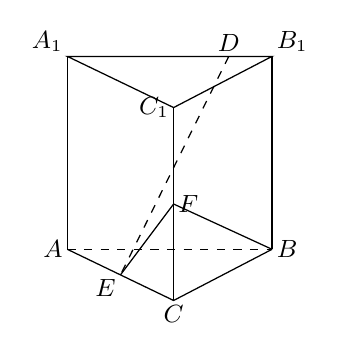
\begin{tikzpicture}[font=\small,line width=0.45pt,
  every node/.style={inner sep=1.5pt}]
  \coordinate (A1) at (0,2.8);  \coordinate (B1) at (2.6,2.8);
  \coordinate (C1) at (1.35,2.15);
  \coordinate (A) at (0,0.35); \coordinate (B) at (2.6,0.35);
  \coordinate (C) at (1.35,-0.30);
  \coordinate (D) at (2.05,2.8);
  \coordinate (E) at (0.675,0.025); \coordinate (F) at (1.35,0.925);
  % 上底、侧棱、下底（遮挡的 AB 为虚线）
  \draw (A1)--(B1)--(C1)--cycle;
  \draw (A1)--(A) (B1)--(B) (C1)--(C);
  \draw[dashed] (A)--(B);
  \draw (A)--(C)--(B);
  % 题设线段
  \draw (B)--(F) (E)--(F);
  \draw[dashed] (D)--(E);
  % 点名
  \node[anchor=south east] at (A1) {$A_1$};
  \node[anchor=south west] at (B1) {$B_1$};
  \node[anchor=east] at (C1) {$C_1$};
  \node[anchor=east] at (A) {$A$};
  \node[anchor=west] at (B) {$B$};
  \node[anchor=north] at (C) {$C$};
  \node[anchor=south] at (D) {$D$};
  \node[anchor=north east] at (E) {$E$};
  \node[anchor=west] at (F) {$F$};
\end{tikzpicture}
\end{center}
\nopagebreak[4]
（1） 证明：$BF\perp DE$。

（2） 当 $B_1D$ 为何值时，面 $BB_1C_1C$ 与面 $DEF$ 所成的二面角正弦值最小？

\end{question}
\begin{question}
\gkti{20}\textbf{（12 分）} 抛物线 $C$ 的顶点为坐标原点 $O$，焦点在 $x$ 轴上，直线 $l:x=1$ 交 $C$ 于 $P$，$Q$ 两点，且 $OP\perp OQ$。已知点 $M(2,0)$，且圆 $M$ 与 $l$ 相切。

（1） 求 $C$，圆 $M$ 的方程。

（2） 设 $A_1$，$A_2$，$A_3$ 是 $C$ 上的三个点，直线 $A_1A_2$，$A_1A_3$ 均与圆 $M$ 相切。判断 $A_2A_3$ 与圆 $M$ 的位置关系，并说明理由。

\end{question}
\begin{question}
\gkti{21}\textbf{（12 分）} 已知 $a>0$ 且 $a\ne1$，函数 $f(x)=\dfrac{x^a}{a^x}\ (x>0)$。

（1） 若 $a=2$，求 $f(x)$ 的单调区间。

（2） 若曲线 $y=f(x)$ 与直线 $y=1$ 有且仅有两个交点，求 $a$ 的取值范围。

\end{question}
\begin{question}
\gkti{22}\textbf{（10 分）选修 4—4：坐标系与参数方程} 

在直角坐标系 $xOy$ 中，以坐标原点为极点，$x$ 轴正半轴为极轴建立极坐标系，曲线 $C$ 的极坐标方程为 $\rho=2\sqrt2\cos\theta$。

（1） 将 $C$ 的极坐标方程化为直角坐标方程。

（2） 设点 $A$ 的直角坐标为 $(1,0)$，$M$ 为 $C$ 上的动点，点 $P$ 满足 $\overrightarrow{AP}=\sqrt2\,\overrightarrow{AM}$。写出 $P$ 的轨迹 $C_1$ 的参数方程，并判断 $C$ 与 $C_1$ 是否有公共点。

\Needspace{0.4\textheight}
\end{question}
\begin{question}
\gkti{23}\textbf{（10 分）选修 4—5：不等式选讲} 

已知函数 $f(x)=|x-2|$，$g(x)=|2x+3|-|2x-1|$。
\nopagebreak[4]
\begin{center}% 2021 全国甲卷理科 23：不等式作图用的空白方格坐标系
% 源图为以原点为中心、横纵各 8 格的网格，只标坐标轴、O 与单位刻度。
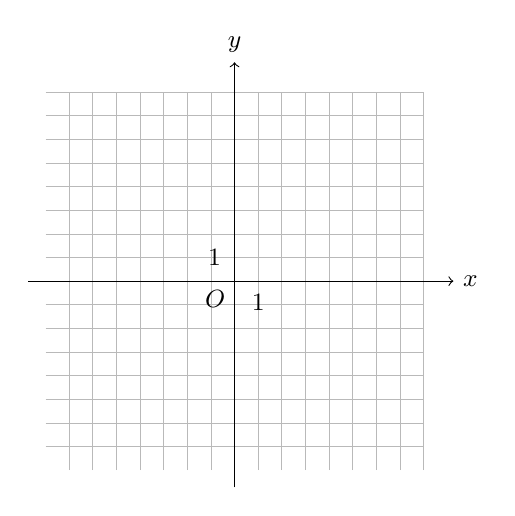
\begin{tikzpicture}[font=\small,line width=0.4pt]
  \def\u{0.30}
  \draw[gray!55,line width=0.25pt] (-2.4,-2.4) grid[step=\u] (2.4,2.4);
  \draw[->] (-2.62,0)--(2.78,0) node[anchor=west] {$x$};
  \draw[->] (0,-2.62)--(0,2.78) node[anchor=south] {$y$};
  \node[anchor=north east,inner sep=2pt] at (-0.04,-0.04) {$O$};
  \node[anchor=north,inner sep=3pt] at (\u,-0.06) {$1$};
  \node[anchor=east,inner sep=3pt] at (-0.06,\u) {$1$};
\end{tikzpicture}
\end{center}
\nopagebreak[4]
（1） 画出 $y=f(x)$ 和 $y=g(x)$ 的图象。

（2） 若 $f(x+a)\geqslant g(x)$，求 $a$ 的取值范围。

\clearpage

\end{question}